%!TEX root = ../PTC-LibUG.tex

\chapter{Symplectic Integration and Splitting}
\label{cha:symplectic.integ}

\index{integrator!splitting elements into integration nodes}
\index{integration node!splitting}
\index{element!splitting into integration nodes}
\index{splitting!elements into integration nodes}
\index{resplitting|see{splitting}}
\index{cutting|see{splitting}}
\index{recutting|see{splitting}}
%
\PTC\ generally attempts to integrate the maps of each magnet using a
symplectic integrator. The current release of \PTC\ supports two exceptions
to explicit symplectic integration: the traveling wave cavity used in linear
accelerators and the pancake type  for fitted B-fields. Support for other
exceptions could be added to be \PTC: exact wigglers and exact helical
dipoles, exact solenoids, etc.

This chapter discusses the elements of \PTC\ amenable to explicit
symplectic integration.


\section{Philosophy}
\label{sec:talman.phil}

\index{integration!philosophy}
\index{integration!steps}
\index{integration!process}
\index{symplectic integration|see{integration}}
\index{Talman, Richard!philosophy for symplectic integration}
%
\PTC's philosophy for symplectic integration, which is based on the work
of Richard Talman,%
\footnote{In the early days of ``kick'' codes, physicists believed that the
drift-kick-drift (D-K-D) kick model was massively inadequate because it
requires a large number of steps to achieve decent convergence and
thus the correct tunes. Such codes were restricted to special applications
such as radiation and spin calculations---Chao's code SLIM. 

The reason for this state of affairs was two-fold. First, a technical reason.
We did not have high-order symplectic integrators. Second, a philosophical
reason. People did not understand their own approaches, which
contradicted the inadequacy of kick codes.

The technical issue was resolved by Ruth and later by a cabal of authors
including Neri, Forest, and finally Yoshida. We can use high-order symplectic
integrators on our usual ``MAD8'' Hamiltonian for the body of the magnet. 

Almost simultaneously, the code TEAPOT emerged from the suffocating
entrails of the SSC-CDG. TEAPOT integrated exactly using a D-K-D
method---or more accurately, a PROT-KICK-PROT method---the combined
function S-bend. TEAPOT was a second-order code restricted to one step
of integration or four strange steps for the IR quadrupoles! (PROT is a drift
in polar coordinates used in S-bend integration and in patching.)

Talman, the principal person pushing TEAPOT, realized that in accelerator
physics the integration step is part of the model. For example, people who
objected to the D-K-D integration method would themselves always use a
single kick for the sextupoles. They would then adjust chromaticities not
based on the thick sextupole model but based on their semi-serious one-kick
representation. Remarkably, the results are acceptable for most machines. 

Talman realized that if he fitted each cell of the SSC to exactly 90 degrees,
the results with one kick per quadrupole would be nearly identical to that of
a ``matrix'' code. Better still, Talman's code---once the magnets are refitted
to achieve a correct machine---could potentially produce the correct physics
for small rings while the standard ``matrix-kick-matrix'' codes could not
because they relied on the small angle approximation.}
involves six steps:
\begin{enumerate}
  \item Split the elements in the lattice into integration nodes%
  \footnote{During tracking, \PTC\ performs an integration step for each
  integration node in the body of an element.}
   using one of \PTC's integration methods. For a list of \PTC's integration methods,
   see Section~\ref{sub:Integration-Methods}.
  \item Fit all the stuff you would normally fit using your matching routines.
  \item Examine the resulting lattice functions and perhaps some short-term
  dynamic aperture.
  \item If your results are satisfactory, reduce the number of integration nodes,
  the sophistication of the integration method, or both.  Then go back to step 1.
  \item If your results are not satisfactory, increase the number of integration
  nodes, the sophistication of the integration method, or both. Then go back to step 1.
  \item After oscillating between steps 4 and 5, make up your mind and
  call that the lattice.
\end{enumerate}

For your particular lattice, store all the information at step 6 so that you do
not have to repeat the process!

In this chapter, we describe step 1 in detail. The other steps depend on
the results you want for your simulation.

\index{Talman, Richard!algorithm}
\index{Talman, Richard!integration process}
\fxnote{Mysterious reference!}
Example 3 in Section~??
%\ref{sub:DNA-Database}
gives an example---the ``Talman algorithm''---of \PTC\ code that performs these steps. 


\subsection{Integration Methods}
\label{sub:Integration-Methods}

\index{integration methods!described}
%
\PTC\ has six integration methods.

\index{drift-kick-drift!integration methods}
\index{kick!integration method}
%
In the drift-kick-drift (D-K-D) case, \PTC\ has three methods of integration:
\begin{itemize}
  \item method 2, the na\"{i}ve second-order method,
  which has one kick per integration step,
  \item method 4, the Ruth-Neri-Yoshida fourth-order method,
  which has three kicks per integration step,
  \item method 6, the Yoshida sixth-order method,
  which has seven kicks per integration step.
\end{itemize}

\fxnote{Al: In trying to figure out the examples, I have made the ``kicks-per-step'' assumptions above based on \'Etienne's comment at Example 3 (see his Word document): ``The number of thin lenses for method 6 is 7 per steps. Method 4 has 3 kicks per steps.'' Is my assumption correct? If not, this text and much of the text describing the examples must be rewritten.}

\index{matrix-kick-matrix!integration methods}
%
In the matrix-kick-matrix (M-K-M) case, \PTC\ also has three methods of integration:
\begin{itemize}
  \item method 1,
  \item method 3,
  \item method 5.
\end{itemize}

\fxnote{Give brief descriptions of methods 1, 3, and 5.}

For more information about integration methods, see Section~\ref{sub:Matrix-Kick-Matrix}.


\section{Splitting Tutorial Source File}

\index{PTC!source file}
\index{source file!splitting tutorial}
\index{splitting!tutorial source file}
\index{z\_ptc\_splitting.f90@\ptc{z\_ptc\_splitting.f90}!splitting tutorial source file}
%
The example code in this chapter is from the tutorial source file \ptc{ptc\_splitting.f90} in \TAref*{splitting}. The line numbers of the code in the examples refer to the line numbers of the code in the appendix.

\fxnote{Add line numbers to \PTC\ code.}


\section{Splitting the Lattice}
\label{sec:splitting.lattice}

\index{integrator!splitting elements into integration nodes}
\index{integration node!splitting}
\index{element!splitting into integration nodes}
\index{splitting!elements into integration nodes}
%
This section describes the routines, global parameters, and arguments
involved in splitting elements in the lattice.


\subsection{Global Parameters}

\index{global parameter!\ptc{resplit\_cutting}}
\index{resplit\_cutting@\ptc{resplit\_cutting}!global parameter}
\index{global parameter!\ptc{sixtrack\_compatible}}
\index{sixtrack\_compatible@\ptc{sixtrack\_compatible}!global parameter}
\index{global parameter!\ptc{radiation\_bend\_split}}
\index{radiation\_bend\_split@\ptc{radiation\_bend\_split}!global parameter}
\index{global parameter!\ptc{fuzzy\_split}}
\index{fuzzy\_split@\ptc{fuzzy\_split}!global parameter}
%
The default values for the global parameters are in {\textit{\textcolor{red}{red
italic }}}type.

Four global parameters are involved in splitting the lattice:
\begin{itemize}
  \item \ptc{resplit\_cutting} (\textit{\textcolor{red}{0}}, 1, or 2)
        For more information, see Section~\ref{sub:LMAX0-Optional-Argument}.
  \item \ptc{sixtrack\_compatible} (true or \textit{\textcolor{red}{false}})
        This global parameter enforces a second-order integrator for all magnets.
  \item \ptc{radiation\_bend\_split} (true or \textit{\textcolor{red}{false}})
        This global parameter splits bends with integration method 2 to improve
        radiation or spin results. For more information about \PTC's methods of
        integration, see Section~\ref{sub:Integration-Methods}.
  \item \ptc{fuzzy\_split} (default to \textit{\textcolor{red}{1.0}})
        If this global parameter is greater than 1.0, \PTC\ lets some magnets with
        slightly too-long integration steps go through,
        i.e., if \ptc{ds<lmax0*fuzzy\_split}.
\end{itemize}


\subsection{Splitting Routines}

\index{splitting!routines}
\index{routines!splitting elements into integration nodes}
\index{routine!\ptc{THIN\_LENS\_RESTART}}
\index{THIN\_LENS\_RESTART@\ptc{THIN\_LENS\_RESTART}!routine}
\index{routine!\ptc{THIN\_LENS\_RESPLIT}}
\index{THIN\_LENS\_RESPLIT@\ptc{THIN\_LENS\_RESPLIT}!routine}
%
Mandatory arguments for the routines are in \ptc{regular black} type.
Optional arguments are in \ptc{\textit{\textcolor{red}{red italic}}} type.

\ptc{THIN\_LENS\_RESTART(R1\textit{\textcolor{red}{,FIB,USEKNOB}})}

This routine resets all magnets to second-order integration with one step. 

\ptc{THIN\_LENS\_RESPLIT(R\textit{\textcolor{red}{,THIN,EVEN,LIM(1:2),LMAX0,XBEND,FIB,USEKNOB}})}

This routine splits all the magnets in the lattice into integration nodes, or \emph{thin lenses}.

To restrict the action of \ptc{THIN\_LENS\_RESTART} and \ptc{THIN\_LENS\_RESPLIT}
to specific fibres or groups of magnets, use the optional arguments \ptc{FIB} and
\ptc{USEKNOB}. For more information, see Section~\ref{sub:Arguments}.


\subsection{Arguments}
\label{sub:Arguments}

This section describes the arguments for  the \ptc{THIN\_LENS\_RESTART} and
\ptc{THIN\_LENS\_RESPLIT} routines.


\subsubsection{R1 or R Argument}

The name of the layout to be split.

\fxnote{Al: Is the above information correct? A commented-out line
of code in the geometry tutorial had a call to \ptc{thin\_lens\_resplit} with \ptc{m\_u\%end} as the first argument.}


\subsubsection{Optional Argument THIN}

The optional argument \ptc{THIN} describes an approximate integrated quadrupole
strength for which a single integration node, or \emph{thin lens}, in the body of an
element should be used. For example, the quadrupoles QF and QD in Example 1 below
have an integrated strength of
\begin{ptccode}
KF L = 0.279309637578521      KD L=-0.197159744173073
\end{ptccode}
 
 
\subsubsection*{Example 1}

For our \ptc{build-psr} layout (see \TPref*{sec:build.psr}), we make following calls:
\begin{ptccode}
CALL MOVE_TO(R1,QF,"QF",POS)
CALL MOVE_TO(R1,QD,"QD",POS)
THIN=0.01D0
LIMITS(1:2)=100000

CALL THIN_LENS_RESPLIT(R1,THIN,LIM=LIMITS)
WRITE(6,*) QF%MAG%NAME,QF%MAG%P%METHOD,QF%MAG%P%NST
WRITE(6,*) QD%MAG%NAME,QD%MAG%P%METHOD,QD%MAG%P%NST
\end{ptccode}

\ptc{NST} is the number of integration steps.

\tref[c]{Results-Example-1} shows the results.

\begin{table}[htdp]
\caption{Results of Example 1.}
\label{tbl:Results-Example-1}
\begin{center}
\begin{tabular}{ccccc} \toprule
  Element  & Method & Steps & Kicks/Step & Total Kicks \\ \midrule
  \ptc{QF} &   2    &   27  &     1      &    27 \\
  \ptc{QD} &   2    &   19  &     1      &    19 \\
  \ptc{B}  &   2    &   15  &     1      &    15 \\ \bottomrule
\end{tabular}
\end{center}
\end{table}

\ptc{KF/THIN} is about 27.9, which is close to the 27 integration steps
that result from Example 1, and \ptc{KD/THIN} is about 19.7, which is
close to the 19 integration steps that result from Example 1. Example 1
behaves as expected: it splits according to quadrupole strength. The method
stayed \ptc{2}, i.e., second-order integrator. This is not efficient if the number 
of steps must be large. Therefore we must teach the splitting algorithm to 
switch to the fourth-order or sixth-order integrator. We discuss how to do this in
Section~\ref{sub:LIM-Optional-Argument}.

In the bend, we also look at the amount of natural horizontal focusing,
vertical focusing, or both. In this example, a small ring with bends of
36 degrees, the bends are unusually strong. The global parameter
\ptc{radiation\_bend\_split} and the optional argument \ptc{xbend} can be used
to affect the bends.


\subsubsection{LIM Optional Argument}
\label{sub:LIM-Optional-Argument}

The optional array \ptc{lim(2)} determines when \PTC\ should choose the
second-order, fourth-order, or sixth-order integration method.

\begin{itemize}
  \item \ptc{lim(1)} > \ptc{KL/THIN}: second-order method,
  \item \ptc{lim(2)} > \ptc{KL/THIN} > \ptc{lim(1)}: fourth-order method,
  \item \ptc{KL/THIN} > \ptc{lim(2)}: sixth-order method.
\end{itemize}

\fxnote{Al: Is the above itemized list correct? \'Etienne's document
has an error at this point. He repeated item 2 as item 3. I have taken my
best guess at what item 3 should be based on the example below. (There's
no guarantee item 2 is correct.)}


\subsubsection*{Example 2}

Let us rerun the previous case with a different limit array:

\begin{ptccode}
THIN = 0.01D0
LIMITS(1) = 8
LIMITS(2) = 24

CALL THIN_LENS_RESPLIT(R1,THIN,LIM=LIMITS)
WRITE(6,*) QF%MAG%NAME, QF%MAG%P%METHOD, QF%MAG%P%NST
WRITE(6,*) QD%MAG%NAME, QD%MAG%P%METHOD, QD%MAG%P%NST
\end{ptccode}

Note that \ptc{KF/THIN}, which is about 27.9, is greater than \ptc{lim(2)}, which
is 24. \ptc{KD/THIN}, which is about 19.7, is less than \ptc{lim(2)}. Both are greater
than \ptc{lim(1)}.

\tref[c]{Results-Example-2} shows the results.
\begin{table}[htdp]
\caption{Results of Example 2.}
\label{tbl:Results-Example-2}
\begin{center}
\begin{tabular}{ccccc} \toprule
  Element  & Method & Steps & Kicks/Step & Total Kicks \\ \midrule
  \ptc{QF} &   6    &   3   &     7      &    21 \\
  \ptc{QD} &   4    &   6   &     3      &    18 \\
  \ptc{B}  &   4    &   5   &     3      &    15 \\ \bottomrule
\end{tabular}
\end{center}
\end{table}

\PTC\ uses integration method~6 for element \ptc{QF}, which results in
three integration steps with seven kicks per step:  a total of 21 kicks.
\PTC\ uses integration method~4 for element \ptc{QD}, which results in
six integration steps with three kicks per step: a total of 18 kicks. As we
can see, the number of kicks has remained more or less constant while
the integration method has increased in order.

\fxnote{Al: Please check my revisions against \'Etienne's Word document. This is the only way I can get his much-smaller table to make sense to me.}


\subsubsection*{Example 3}

\index{Talman, Richard!algorithm}
\index{Talman, Richard!integration process}
\index{integration!steps}
\index{integration!process}
\index{tune!computing}
\index{beta function!computing}
\index{closed orbit!computing}
\index{chromaticity!computing}
\index{stability!computing}
%
This \PTC\ code is an example of the six-step \PTC\ philosophy for splitting
(see \Sref{talman.phil}), which we are calling the ``Talman algorithm''.
The example reuses Example 2's limit array.

\fxnote{Al: Are the first two lines of code duplicated? It looks that 
way to me.}

\begin{ptccode}
!!!! TALMAN ALGORITHM !!!!! !!!!!  EXAMPLE 3
WRITE(6,*) "  "
WRITE(6,*) "!!!! TALMAN ALGORITHM !!!!! !!!!!  EXAMPLE 3"
WRITE(6,*) "  "

! PART 1A
THIN=0.001D0  ~! CUT LIKE CRAZY
CALL THIN_LENS_RESPLIT(R1,THIN,LIM=LIMITS)
!!! PTC COMMAND FILE: COULD BE A MAD-X COMMAND OR WHATEVER
! COMPUTING TUNE AND BETA AROUND THE RING

! PART 1B
CALL READ_PTC_COMMAND77("FILL_BETA0.TXT")
WRITE(6,*) "  "
WRITE(6,*) " NOW REDUCING THE NUMBER OF STEPS AND REFITTING "
WRITE(6,*) "  "
! PART 2
DO I=0,2
THIN=0.01D0+I*0.03

! PART 2A
CALL THIN_LENS_RESPLIT(R1,THIN,LIM=LIMITS) ! REDUCING NUMBER OF CUTS
! FITTING TO PREVIOUS TUNES

! PART 2B
CALL READ_PTC_COMMAND77("FIT_TO_BETA0_RESULTS.TXT")
! COMPUTING DBETA/BETA AROUND THE RING

! PART 2C
CALL READ_PTC_COMMAND77("FILL_BETA1.TXT")
ENDDO
\end{ptccode}

Example 3 uses the limits from Example 2: \ptc{lim(1)} of 8 and \ptc{lim(2)} of 24 with
\ptc{THIN=0.001D0}. \ptc{KF/THIN} is now about 279, and \ptc{KD/THIN} is about 197.
Both are much greater than \ptc{lim(2)}. \PTC\ will use integration method 6, which has 
seven kicks per integration step.

\tref[c]{Results-Example-3} and the list below show the results for Part 1A of Example 3.

\begin{table}[htdp]
\caption{Results of Example 3 for Part 1A.}
\label{tbl:Results-Example-3}
\begin{center}
\begin{tabular}{ccc} \toprule
  Method & ?  & ? \\ \midrule
    2    & 40 & 40 \\
    4    &  0 &  0 \\
    6    & 30 & 6230 \\ \bottomrule
\end{tabular}
\end{center}
\end{table}

\begin{itemize}
  \item Number of slices: 6270.
  \item Total NST: 930.
  \item Total NST due to Bend Closed Orbit: 0.
  \item Biggest ds: 0.115885454545455.
\end{itemize}

The quadrupoles and the dipoles are split using integration method 6 with a grand total of 6240 slices.

\fxnote{Al: I don't understand where the numbers are coming from in the table and the list. What are the two columns in the table: quadrupoles and dipoles? QF and QD? If NST is another name for ``number of integration steps'', why is the number of slices different than the total NST? (I have come to the conclusion that ``slices'' represents kicks rather than steps. Is that correct?) What does ``Bend Closed Orbit'' refer to?}

In Part 1B, compute the tunes and betas around the ring. The fractional tunes are: 
\begin{ptccode}
0.142192063715077      0.854078356314425
\end{ptccode}

And the betas are stored for future use.

In Part 2A, the magnet is resplit less and less finely, the tune is refitted, and finally the
delta beta around the ring is estimated as a measure of the splitting adequacy. 

The results for \ptc{THIN  = 0.01} are:
\begin{itemize}
  \item \ptc{<DBETA/BETA> =   4.025629639896395E-006}
  \item \ptc{MAXIMUM OF DBETA/BETA =   6.034509389788590E-006}
\end{itemize}

The results for \ptc{THIN  = 0.04} are:
\begin{itemize}
  \item  \ptc{<DBETA/BETA> =   2.065365900468319E-003}
   \item \ptc{MAXIMUM OF DBETA/BETA =   4.014532098810251E-003}
\end{itemize}

The results for \ptc{THIN  = 0.07} are:
\begin{itemize}
  \item  \ptc{<DBETA/BETA> =   5.779446473894797E-003}
  \item  \ptc{MAXIMUM OF DBETA/BETA =   1.068563516341058E-002}
\end{itemize}

One can also look at the chromaticities. For example, the chromaticities
at the beginning were:
\begin{ptccode}
-2.87009384223620       -2.03916389491785
\end{ptccode}

At the end, the chromaticities are:
\begin{ptccode}
-2.86244921970493       -2.03671376872069
\end{ptccode}

At this point, we can freeze the lattice for good. Of course refitting the tune
was only an example: in other lattices we may want to rematch a more
complete set of properties: dispersion, alphas, phase advances, etc.


\subsubsection{XBEND Optional Argument}

\index{global parameter!\ptc{exact\_model}}
\index{exact\_model@\ptc{exact\_model}!global parameter}
%
This section discusses usage of the \ptc{XBEND} optional argument when 
\ptc{exact=.true.}

The lattice uses sector bends. Because this is an ideal lattice, the tune should
be the same regardless of whether with \ptc{exact\_model=true} or \ptc{false}.
Therefore we will fit to the same tune as before, passing it through the same
algorithm.


\subsubsection*{Example 4}

\begin{ptccode}
WRITE(6,*) "  "
WRITE(6,*) "!!!! SBEND ORBIT SMALL PROBLEM !!!!! !!!!!  EXAMPLE 4"
WRITE(6,*) "  "

CALL APPEND_EMPTY_LAYOUT(M_U)  ! NUMBER 2 
CALL SET_UP(M_U%END)
R1=>M_U%END

EXACT=.TRUE.
METHOD=DRIFT_KICK_DRIFT
CALL RUN_PSR(R1,EXACT,METHOD)

WRITE(6,*) "  "
WRITE(6,*) " NOW REDUCING THE NUMBER OF STEPS AND REFITTING "
WRITE(6,*) "  "
DO I=0,2
 THIN=0.01D0+I*0.03
 CALL THIN_LENS_RESPLIT(R1,THIN,LIM=LIMITS) ! REDUCING NUMBER OF CUTS
 ! FITTING TO PREVIOUS TUNES
CALL READ_PTC_COMMAND77("FIT_TO_BETA0_RESULTS_2.TXT") 
  ! COMPUTING DBETA/BETA AROUND THE RING 
CALL READ_PTC_COMMAND77("FILL_BETA1_2.TXT")
ENDDO
\end{ptccode}

The results of the last iteration for the closed orbit are:

\begin{ptccode}
 -3.129618316516444E-002  3.357101188909470E-003  0.000000000000000E+000
  0.000000000000000E+000  0.000000000000000E+000  0.000000000000000E+000
\end{ptccode}

The results of the last iteration for the stability is T.

The results of the last iteration for the tunes are:
\begin{ptccode}
0.142192063715077       0.854078356314425
\end{ptccode}

In addition:
\begin{itemize}
  \item \ptc{<DBETA/BETA> =  1.184251326377263E-002}
  \item \ptc{MAXIMUM OF DBETA/BETA =   2.032348481520253E-002}
\end{itemize}

We notice that the closed orbit is wild and that the fluctuation of the beta functions
is twice as big as before. 

This problem can be alleviated by enforcing a finer split of the bend. This is done by
setting the  \ptc{XBEND} argument to some small value that corresponds approximately
to the norm of the residual orbit.


\subsubsection*{Example 5}

In example 5, the splitting line is replaced by this one:

\begin{ptccode}
CALL THIN_LENS_RESPLIT(R1,THIN,LIM=LIMITS,XBEND=1.D-4)
\end{ptccode}

The results of the final iteration steps for the closed orbit are:
\begin{ptccode}
 -3.377915412576128E-003  3.670253104757456E-004  0.000000000000000E+000
  0.000000000000000E+000  0.000000000000000E+000  0.000000000000000E+000
\end{ptccode}

The results of the final iteration for the stability is T.

The results of the final iteration for the tunes are:
\begin{ptccode}
0.142192063715077       0.854078356314425
\end{ptccode}

In addition:
\begin{itemize}
  \item \ptc{<DBETA/BETA> =  3.542348342695508E-003}
  \item \ptc{MAXIMUM OF DBETA/BETA =  5.551255781973659E-003}
\end{itemize}


\subsubsection{EVEN Optional Argument}

There are three possibilities for the \ptc{EVEN} optional argument:
\begin{itemize}
  \item \ptc{EVEN=true} enforces an even split,
  \item \ptc{EVEN=false} enforces an odd split,
  \item \ptc{EVEN} is not in the call statement: an even or odd split is acceptable.
\end{itemize}


\subsubsection*{Example 6}

\ptc{EVEN=true} is important if the motion must be observed at the center of a
magnet. This is useful during matching procedures in particular.

The data in \tref{Results-Example-6-NONE} show
the ``indifferent'' splitting. \ptc{T1} is a pointer to the integration node
at the beginning of the fibre. \ptc{TM} points to the center if it exists.
\ptc{T2} points to the end of the fibre. \ptc{TM} and \ptc{T1} are identical
when the number of steps is odd; there is no center of the magnet,
and by default \ptc{TM} points to \ptc{T1}.

\begin{table}[htdp]
\caption{Results of Example 6 when \ptc{even} is not specified.}
\label{tbl:Results-Example-6-NONE}
\begin{center}
\begin{tabular}{cccccc} \toprule
   Name    & Method & Steps & \ptc{T1\%pos} & \ptc{TM\%pos} & \ptc{T2\%pos} \\ \midrule
  \ptc{QF} &   6    &   3   &      35       &      35       &      41 \\
  \ptc{QD} &   4    &   6   &      52       &      57       &      61 \\
  \ptc{B}  &   4    &   5   &      67       &      67       &      75 \\ \bottomrule
\end{tabular}
\end{center}
\end{table}
 
The data in \tref{Results-Example-6-EVEN} shows that when
we use \ptc{EVEN=true}, \ptc{TM} is always different from \ptc{T1}. \ptc{TM}
points directly at the center of the magnet.

\begin{table}[htdp]
\caption{Results of Example 6 when \ptc{even=.true.}}
\label{tbl:Results-Example-6-EVEN}
\begin{center}
\begin{tabular}{cccccc} \toprule
   Name    & Method & Steps & \ptc{T1\%pos} & \ptc{TM\%pos} & \ptc{T2\%pos} \\ \midrule
  \ptc{QF} &   6    &   4   &      39       &      43       &      46 \\
  \ptc{QD} &   4    &   6   &      59       &      64       &      68 \\
  \ptc{B}  &   4    &   6   &      75       &      80       &      84 \\ \bottomrule
\end{tabular}
\end{center}
\end{table}


\subsubsection{LMAX0 Optional Argument}
\label{sub:LMAX0-Optional-Argument}

The \ptc{lmax0} optional argument must be used in conjunction with the
\ptc{resplit\_cutting} global parameter set to \ptc{1} or \ptc{2}. The \ptc{resplit\_cutting}
global parameter is normally defaulted to zero.

If \ptc{resplit\_cutting=1}, the ordinary magnets are left as is. However, the
drifts are split so that the maximum length of an integration node cannot exceed
\ptc{lmax0}.


\subsubsection*{Example 7}

\begin{ptccode}
call move_to(r1,d1,"D1",pos)
call move_to(r1,d1_next,"D1",pos)
call move_to(r1,d2,1) !!! Put the pointer for search back at position 1
call move_to(r1,d2,"D2",pos)
call move_to(r1,qf,"QF",pos)
call move_to(r1,qd,"QD",pos)
call move_to(r1,b,"B",pos)
resplit_cutting=1
call THIN_LENS_restart(r1)
thin=0.01d0
CALL THIN_LENS_resplit(R1,THIN,even=.true.,lmax0=0.05d0,xbend=1.d-4)
\end{ptccode}

\tref[c]{Results-Example-7-1} shows the results of the above run.

\begin{table}[ht]\forcerectofloat
\caption{Results of Example 7 for \ptc{resplit\_cutting=1}.}
\label{tbl:Results-Example-7-1}
\begin{center}
\begin{tabular}{cccccc} \toprule
   Name    & Method & Steps & \ptc{T1\%pos} & \ptc{TM\%pos} & \ptc{T2\%pos} \\ \midrule
  \ptc{D1} &   2    &  46   &       1       &      26       &     102 \\
  \ptc{D1} &   2    &  46   &     103       &      26       &     152 \\
  \ptc{D2} &   2    &  10   &      57       &      64       &      70 \\
  \ptc{QF} &   6    &   4   &      95       &      99       &     102 \\
  \ptc{QD} &   6    &   2   &     203       &     206       &     208 \\
  \ptc{B}  &   4    &   6   &     223       &     228       &     232 \\ \bottomrule
\end{tabular}
\end{center}
\end{table}

Notice that only the drifts \ptc{D1} and \ptc{D2} were split.

If \ptc{resplit\_cutting=2}, then all the magnets and the drifts are split to
achieve a maximum length of \ptc{lmax0}. This is useful in space-charge
calculations. See \tref{Results-Example-7-2}.

\begin{table}[htb]
\caption{Results of Example 7 for \ptc{resplit\_cutting=2}.}
\label{tbl:Results-Example-7-2}
\begin{center}
\begin{tabular}{cccccc} \toprule
   Name    & Method & Steps & \ptc{T1\%pos} & \ptc{TM\%pos} & \ptc{T2\%pos} \\ \midrule
  \ptc{D1} &   2    &  46   &       1       &      26       &     166 \\
  \ptc{D1} &   2    &  46   &     167       &      26       &     216 \\
  \ptc{D2} &   2    &  10   &      67       &      74       &      80 \\
  \ptc{QF} &   6    &  12   &     151       &     159       &     166 \\
  \ptc{QD} &   6    &  12   &     267       &     275       &     282 \\
  \ptc{B}  &   4    &  52   &     297       &     325       &     352 \\ \bottomrule
\end{tabular}
\end{center}
\end{table}

Now all the magnets are split.


\subsubsection{FIB Optional Argument}

Continuing with the previous example, we make the following call.


\subsubsection*{Example 8}

\begin{ptccode}
WRITE(6,*) "!!!! FIB KEYWORD  !!!!! !!!!!  EXAMPLE 8"
CALL THIN_LENS_RESTART(R1)
CALL THIN_LENS_RESPLIT(R1,THIN,EVEN=.TRUE.,LMAX0=0.005D0,XBEND=1.D-4,FIB=D1_NEXT)
\end{ptccode}

\tref[c]{Results-Example-8} shows the results.

\begin{table}[htb]
\caption{Results of Example 8.}
\label{tbl:Results-Example-8}
\begin{center}
\begin{tabular}{cccccc} \toprule
   Name    & Method & Steps & \ptc{T1\%pos} & \ptc{TM\%pos} & \ptc{T2\%pos} \\ \midrule
  \ptc{D1} &   2    &  46   &       1       &      26       &      50 \\
  \emph{D1}&\emph{2}&\emph{458}&\emph{167}  &\emph{26}      &\emph{628} \\
  \ptc{D2} &   2    &  10   &      67       &      74       &      80 \\
  \ptc{QF} &   6    &  12   &     151       &     159       &     166 \\
  \ptc{QD} &   6    &  12   &     679       &     687       &     694 \\
  \ptc{B}  &   4    &  52   &     709       &     737       &     764 \\ \bottomrule
\end{tabular}
\end{center}
\end{table}

Only the fibre \ptc{D1\_NEXT} is affected. All the others are left intact.
This allows the splitting of a single fibre.


\subsubsection{USEKNOB Optional Argument}

\index{knob!using}
We can use the type \ptc{pol\_block} to produce a splitting of the lattice.


\subsubsection*{Example 9}

\begin{ptccode}
FAM=0
FAM%NAME="D1"
R1=FAM
CALL THIN_LENS_RESTART(R1) ! PUTS BACK METHOD =2 AND NST=1 EVERYWHERE
CALL THIN_LENS_RESPLIT(R1,THIN,EVEN=.TRUE.,LMAX0=0.005D0,XBEND=1.D-4,
  USEKNOB=.TRUE.)
\end{ptccode}

If \ptc{useknob} is true, then the magnets with the knob flag ``on'' are split, assuming
no other flags prevent it. In this particular case, \ptc{resplit\_cutting=2}, therefore, the
drifts will be split on the basis of \ptc{LMAX0=0.005D0}.

\tref[c]{Results-Example-9-TRUE} shows the results.

\begin{table}[htdp]
\caption{Results of Example 9 when \ptc{useknob=.true.}}
\label{tbl:Results-Example-9-TRUE}
\begin{center}
\begin{tabular}{cccccc} \toprule
   Name    & Method & Steps & \ptc{T1\%pos} & \ptc{TM\%pos} & \ptc{T2\%pos} \\ \midrule
  \emph{D1}&\emph{2}&\emph{458}&\emph{1}    &\emph{232}     &\emph{462} \\
  \emph{D1}&\emph{2}&\emph{458}&\emph{488}  &\emph{232}     &\emph{949} \\
  \ptc{D2} &   2    &   1   &     468       &     468       &     472 \\
  \ptc{QF} &   2    &   1   &     483       &     483       &     487 \\
  \ptc{QD} &   2    &   1   &    1412       &    1412       &    1416 \\
  \ptc{B}  &   2    &   1   &    1422       &    1422       &    1426 \\ \bottomrule
\end{tabular}
\end{center}
\end{table}

If we perform the same call with \ptc{useknob=.false.}, then the magnets
with \ptc{knob=true} are masked and the other magnets are split.

\begin{ptccode}
CALL THIN_LENS_RESPLIT(R1,THIN,EVEN=.TRUE.,LMAX0=0.005D0,XBEND=1.D-4,
  USEKNOB=.FALSE.)
\end{ptccode}

\tref[c]{Results-Example-9-FALSE} shows the results.

\begin{table}[htdp]
\caption{Results of Example 9 when \ptc{useknob=.false.}}
\label{tbl:Results-Example-9-FALSE}
\begin{center}
\begin{tabular}{cccccc} \toprule
   Name    & Method & Steps & \ptc{T1\%pos} & \ptc{TM\%pos} & \ptc{T2\%pos} \\ \midrule
  \ptc{D1} &   2    &   1   &       1       &       1       &       5 \\
  \ptc{D1} &   2    &   1   &     924       &       1       &     928 \\
  \emph{D2}&\emph{2}& \emph{92}& \emph{112} & \emph{160}    & \emph{207} \\
  \emph{QF}&\emph{6}&\emph{102}& \emph{818} & \emph{871}    & \emph{923} \\
  \emph{QD}&\emph{6}&\emph{102}& \emph{934} & \emph{987}    &\emph{1039} \\
  \emph{B} &\emph{4}&\emph{510}&\emph{1136} &\emph{1393}    &\emph{1649} \\ \bottomrule
\end{tabular}
\end{center}
\end{table}

\section{Other Splitting Routines}

\index{routines!splitting elements into integration nodes}
\index{splitting!routines}
\index{integration methods!described}
%
This section discusses \PTC\ integration methods 1, 3, and 5.


\subsection{Splitting a Single Fibre}

\index{routine!\ptc{RECUT\_KIND7\_ONE}}
\index{RECUT\_KIND7\_ONE@\ptc{RECUT\_KIND7\_ONE}!routine}
This routine splits one fibre.

\ptc{RECUT\_KIND7\_ONE(FIBRE,LMAX0,DRIFT)}

In the presence of space charge or for other reasons, it may be more
important to observe the beam at many locations ``approximately'' than
to use a high-order integration method.

\PTC\ provides integration method 1 for certain magnets.


\subsubsection{Drift-Kick-Drift: Strict Talman Interpretation}

\index{Talman, Richard!strict interpretation of drift-kick-drift}
\index{global parameter!\ptc{exact\_model}}
\index{exact\_model@\ptc{exact\_model}!global parameter}
For this type of algorithm, the \ptc{exact\_model = true} and the
\ptc{exact\_model = false} can be switched into method 1 if and only if
the original method was method 2, i.e., second-order integrator.
Basically, negative propagators (drifts) are not acceptable: this is the
strict Talman interpretation to which \PTC\ does not adhere except in the
case of switching to integration method 1.

\fref[c]{Drift-kick-drift} shows a pictorial example.

\begin{figure}[ht]
  \centering
  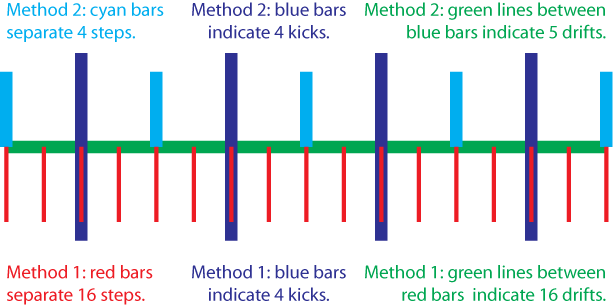
\includegraphics{illustrations/recutDKD}
  \caption{Drift-kick-drift for integration methods 1 and 2.}
  \label{fig:Drift-kick-drift}
\end{figure}

The blue bars and green lines represent the original drift-kick-drift of integration
method 2. The figure shows four kicks and five drifts. There
are four steps, separated by the cyan bars. The new integration method 1
split is simply a splitting of the drifts. There are now 16 drifts (but still 
four kicks). Obviously, the results should be the same to machine precision. 

Example with the 36-degree bend of the PSR (Los Alamos):

\begin{ptccode}
BE  = SBEND("B", 2.54948D0, TWOPI*36.D0/360.D0);
  X=0.001D0
  CALL TRACK(BE,X,DEFAULT)
  WRITE(6,*) BE%MAG%P%METHOD,BE%MAG%P%NST
  WRITE(6,*) X
    CALL RECUT_KIND7_ONE(BE,2.54948D0/16,.FALSE.)
X=0.001D0
  CALL TRACK(BE,X,DEFAULT)
  WRITE(6,*) BE%MAG%P%METHOD,BE%MAG%P%NST
  WRITE(6,*) X
X=0.001D0
  CALL ALLOC(Y)
  Y=X
  CALL TRACK(BE,Y,DEFAULT)
  X=Y
  WRITE(6,*) BE%MAG%P%METHOD,BE%MAG%P%NST
  WRITE(6,*) X
  PAUSE 888
\end{ptccode}

Integration results are:

\begin{ptccode}
     2      4      ------ ! ORIGINAL METHOD AND NUMBER OF STEPS
3.962104445927857E-003  1.253543855340728E-003  3.546933066933068E-003
1.000000000000000E-003  1.000000000000000E-003  2.523695791724136E-003
     1     16
3.962104445927856E-003  1.253543855340728E-003  3.546933066933066E-003
1.000000000000000E-003  1.000000000000000E-003  2.523695791724136E-003
     1     16
3.962104445927856E-003  1.253543855340728E-003  3.546933066933066E-003
1.000000000000000E-003  1.000000000000000E-003  2.523695791724136E-003
\end{ptccode}

Note that method 2 has four integration steps, and method 1 has 16 integration steps.
A larger number of integration steps for method 1 does not change the accuracy.


\subsubsection{Matrix-Kick-Matrix}
\label{sub:Matrix-Kick-Matrix}

\index{integration methods!described}
\index{matrix-kick-matrix!integration methods}
\index{kick!integration method}
%
Integration methods 2, 4, and 6 switching to methods 1, 3, and 5.

\fxnote{Al: I would like to turn the above phrase into a sentence, but I'm not sure what it is saying. In certain circumstances, does \PTC\ use method 1 in place of method 2, method 3 in place of method 4, and method 5 in place of method 6? If so, what are the circumstances?}

\PTC\ has a matrix-kick-matrix method where the matrix is energy independent.
The delta dependence is buried in the kick.

Our comments here apply to \ptc{exact\_model=.false.}

Integration methods 2, 4, and 6---shown in \fref{Matrix-kick-matrix}---always
split the integration step using matrices of equal length. These methods are the so-called
biased integration methods. Although they have existed in accelerators since the days of
SSC, recently they have been discussed at length by McLachlan and also by Laskar and
Robutel.

\fxnote{Al: Should ``existed in accelerators'' be ``existed in accelerator-modeling codes''?}

\begin{figure}[ht]
  \centering
  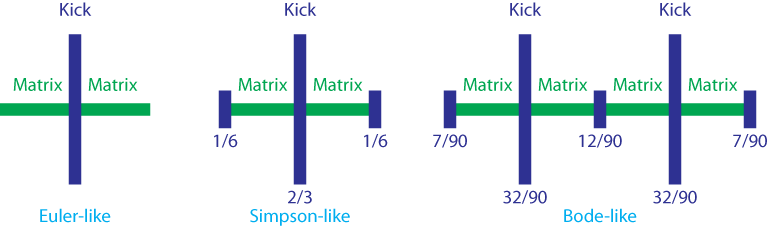
\includegraphics{illustrations/recutMKM}
  \caption{Matrix-kick-matrix for integration methods 2, 4, and 6.}
  \label{fig:Matrix-kick-matrix}
\end{figure}

In accelerators, integration methods 2, 4, and 6 have the advantage of producing
the ``exact'' tune for a typical ideal machine. The effect of the matrix on the kicks is
of order 2, 4, or 6, although all three methods are truly second-order integrators
strictly speaking---the word \emph{biased} refers to this uneven way of ordering
the perturbation due to the kicks Hamiltonian that produced the matrices.

Let us retry the above example with the Bode-like integrator:

\begin{ptccode}
     6      4     ------ ! ORIGINAL METHOD AND NUMBER OF STEPS
3.966179536791447E-003  1.252157150179758E-003  3.546933066933068E-003
1.000000000000000E-003  1.000000000000000E-003  2.529326133576445E-003
     5     16
3.966179536791447E-003  1.252157150179758E-003  3.546933066933068E-003
1.000000000000000E-003  1.000000000000000E-003  2.529326133576445E-003
     5     16
3.966179536791447E-003  1.252157150179758E-003  3.546933066933068E-003
1.000000000000000E-003  1.000000000000000E-003  2.529326133576445E-003
\end{ptccode}

Please note that \ptc{exact\_model=true} works only with straight elements if the matrix-kick-matrix
method (kind7) is selected. Bends should use the drift-kick-drift method (integration method 2) if
 \ptc{exact\_model=true}.
 
\fxnote{Al: \'Etienne's text in his Word document is: ``bends should be of the drift-kick-drift (method 2) if \ptc{exact\_model=true}.'' I've edited his text, but I'm not sure whether he is talking about only method 2 or about methods 2, 4, and 6.}


\subsubsection{Drifts}

\index{routine!\ptc{RECUT\_KIND7\_ONE}}
\index{RECUT\_KIND7\_ONE@\ptc{RECUT\_KIND7\_ONE}!routine}
\index{splitting!drifts}
%
Drifts can be split using:

\ptc{RECUT\_KIND7\_ONE(D1,0.45D0/16.D0,.TRUE.)}


\subsection{Splitting an Entire Lattice}

\index{routine!\ptc{RECUT\_KIND7\_ONE}}
\index{RECUT\_KIND7\_ONE@\ptc{RECUT\_KIND7\_ONE}!routine}
\index{splitting!lattices}
%
This routine applies \ptc{RECUT\_KIND7\_ONE} over the entire layout.

\ptc{RECUT\_KIND7(LAYOUT,LMAX0,DRIFT)}

\endinput
